%========================%
%        Preamble        %
%========================%
\documentclass[12pt]{amsart}

    %========================%
%        Packages        %
%========================%

\usepackage[utf8]{inputenc}
%\usepackage{amsmath}    % Included in amsart package
%\usepackage{amsthm}     % 
\usepackage{amssymb}      % 
\usepackage{mathtools}      % Paired Limiter Macros
% \usepackage{mdframed}       % boxes for theorem
\usepackage{enumitem}     % Continuous numbering of lists
\usepackage[hidelinks]{hyperref}
\usepackage{tikz}
\usetikzlibrary{positioning}
\usepackage{blindtext}
\usepackage{graphicx}
\usepackage{float}

%========================% 
%          Title         %
%========================% 
\title{Chapters 27 and 28 Notes}
\author{Anish Sundaram}
\date{\today}

%========================% 
%        Theorems        %
%========================% 
\theoremstyle{definition}
\newtheorem{theorem}{Theorem}  % Boxed theorems
\newtheorem{definition}{Definition} % Definitions
\newtheorem{example}{Example}       %
\newtheorem{algorithm}{Algorithm}
\newtheorem*{proof*}{Proof}         % non-numbered
\newtheorem*{remark}{Remark}        %
\numberwithin{equation}{theorem}    % Local equation numbering

\setcounter{tocdepth}{3}      % Show subsubsections in contents

%========================% 
%        Macros          %
%========================% 
\DeclarePairedDelimiter\abs{\lvert}{\rvert}  % Vertical bars
\DeclarePairedDelimiter\norm{\lVert}{\rVert} % Double vertical bars
\newcommand{\drawvec}[1]{                    % matrices on one line
    \begin{bmatrix}
        #1
    \end{bmatrix}
}


% \begin{figure}[H]
%     \centering
%     \includegraphics[width=5in]{global-carbon-cycle.png}
%     \caption{The Global Carbon Cycle}
%     \label{global-carbon-cycle}
% \end{figure}

%========================% 
%         Document       %
%========================% 
\begin{document}

\maketitle

\tableofcontents

\section*{27 Magnetic Field and Magnetic Forces}

But the \textit{fundamental} nature of magnetism is the interaction of moving 
electric charges. Unlike electric forces, which act on electric charges 
whether they are moving or not, magnetic forces act only on \textit{moving charges}.

\subsection*{27.1 Magnetism}

\begin{remark}
    The earth itself is a magnet. Its north geographic pole is close to a magnetic south pole, which is why the north pole of a compass needle points north. The earth’s magnetic axis is not quite parallel to its geographic axis (the axis of ro- tation), so a compass reading deviates somewhat from geographic north. This deviation, which varies with location, is called \textit{magnetic declination or magnetic variation.}
\end{remark}

\begin{remark}
     While isolated positive and negative charges exist, there is no experimental evidence that one isolated magnetic pole exists; poles always appear in pairs. If a bar magnet is broken in two, each broken end becomes a pole 
\end{remark}

\begin{figure}[H]
    \centering
    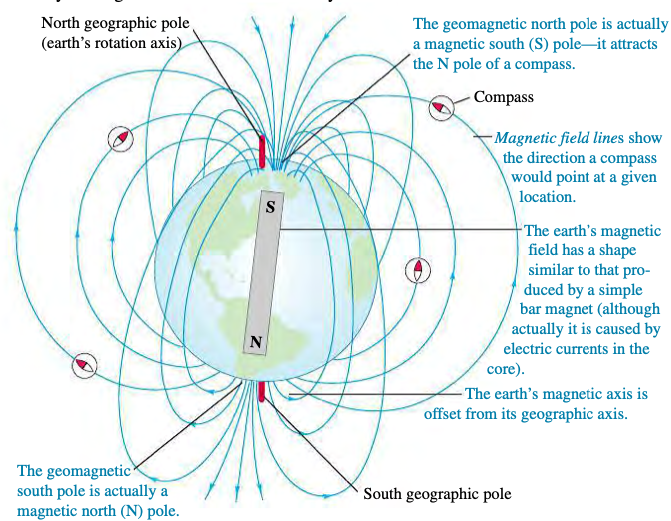
\includegraphics[width=3in]{Media/Magnetism.png}
    \caption{Depiction of Magnetic Field}
    \label{Depiction of Magnetic Field}
\end{figure}

\subsection*{27.2 Magnetic Field}

\begin{definition}
    \textbf{Summary of Electric interactions}:
    \begin{enumerate}
        \item A distribution of electric charge creates an electric field $\vec{E}$ in the surrounding space.
        \item The electric field exerts a force $\vec{F} = q\vec{E}$ on any other charge q that is present in the field.
    \end{enumerate}
\end{definition}

\begin{definition}
    \textbf{Summary of Magnetic interactions}:
    \begin{enumerate}
        \item A moving charge or a current creates a \textbf{magnetic field (B)} in the surrounding
        space (in addition to its \textit{electric} field).
        \item  The magnetic field exerts a force $\vec{F}$ on any other moving charge or current that is present in the field.
    \end{enumerate}

    Magnetic Field strength can be found by the equation 
    $$B = \frac{\mu_0I}{2\pi r}$$ where $\mu_0$ is the permitivity of free space($4\pi \cdot 10^{-7}$ $T\cdot m/A$) and $r$ is the seperation.

    \begin{remark}
        Like electric field, magnetic field is a vector field--that is, a vector quantity associated with each point in space. We will use the symbol $\vec{B}$ for magnetic field.
    \end{remark}
\end{definition}

\begin{figure}[H]
    \centering
    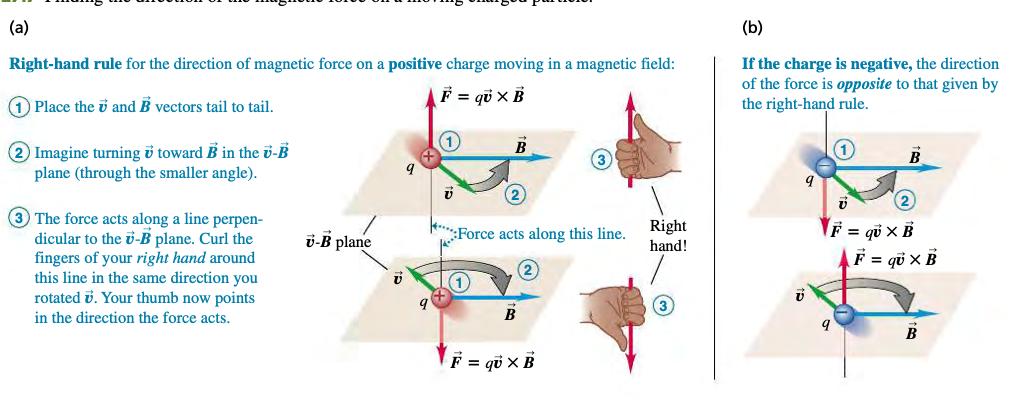
\includegraphics[width=3in]{Media/RHR.png}
    \caption{Right-Hand Rule}
    \label{Right-Hand Rule}
\end{figure}


\subsubsection*{27.2.1 Magnetic Forces on Moving Charges}

\begin{definition}
    \textbf{Key Characteristics of Magnetic Force on Moving Charges}:
    \begin{enumerate}
        \item Force Magnitude is proportional to the magnitude of the charge.
        \item The magnitude of the force is also propor- tional to the magnitude, or “strength,” of the field.
        \item The magnetic force depends on the particle’s
        velocity.
        \item The magnetic force $\vec{F}$ does not have the same direction as the magnetic field $\vec{B}$ but instead is always perpendicular to both $\vec{B}$ and the velocity $\vec{v}$. 
    \end{enumerate}
    The Magnetic force can be found by the equation $$F = |q|v \times B = |q|vBsin\phi$$ where $\phi$ is the angle between the direction of velocity and direction of the magnetic field and the magnitude is measured in teslas ($1T = 1N/A \cdot m$) or in Gauss(1G = $10^{-4}$T)
    \begin{remark}
        The magnetic field of the earth is $10^{-4}$T 1 Gauss.
    \end{remark}
\end{definition}

\begin{remark}
    When a charged particle moves through a region of space where both electric and magnetic fields are present, \textit{both fields exert forces on the particle}. The total force $\vec{F}$ is the vector sum of the electric and magnetic forces: $$\vec{F}=q(\vec{E} + \vec{v}\times \vec{B})$$
\end{remark}

\subsection*{27.3 Magnetic Field Lines and Magnetic Flux}

\begin{definition}
    \textbf{Magnetic Field Lines}:
    Just like an electric field, a magnetic field can be represented through field lines. The more lines there are in a given area the stronger the field , and they never intersect. Magnetic Field Lines are not lines of force, just direction.
\end{definition}

\begin{definition}
    \textbf{Magnetic Flux($\Phi_B$)}:
    A measurement of the total magnetic field which passes through a given area. The total magnetic flux through the surface is the sum of the contributions from the individual area elements. Can be found using the following equation:
    $$\Phi_B = \int B cos\phi dA = \int\vec{B}\cdot d \vec{A}$$
    Magnetic Flux is scalar and its units are Weber(1 Wb = 1 $T\cdot m^2$ = 1 $N\cdot m/A$)

\end{definition}

\subsection*{27.4 Motion of Charged Particles in a Magnetic Field}

\begin{remark}
    Motion of a charged particle under the action of a magnetic field alone is always motion with constant speed.
\end{remark}

\begin{remark}
    When velocity and magnetic field are perpendicular, the particle exhibits circular motion. This relation is shown by $$F = |q|vb = m\frac{v^2}{R}$$ whose radius can be found by $$R = \frac{mv}{|q|B}$$ and whose angular speed can be found by $$\omega = \frac{v}{r} = \frac{|q|B}{m}$$
\end{remark}

\end{document}